
\usepackage[T1]{fontenc}
\usepackage{mathptmx}
\usepackage[scaled=.90]{helvet}
\usepackage{courier}

\usepackage{beamerthemesplit}
\usepackage{verbatim}
\usepackage{hyperref}
\usepackage{listings}
\lstset{language=Perl,basicstyle=\footnotesize,tabsize=3,showstringspaces=false}

\title{Modern PerlCommerce}
\author[racke]{Stefan Hornburg (Racke)\\ \texttt{racke@linuxia.de}}
\date[]{Perl-Mongers Hamburg, 5th December 2011}

\begin{document}
\maketitle{}

\begin{frame}
  \titlepage
\end{frame}

\tableofcontents

\section{Modern PerlCommerce}
In this presentation I'm going to introduce you to our new project
called Nitesi. It's the successor of Interchange, which is a Ecommerce
open source software in Perl being around for a long time.

\begin{frame}{Nitesi}
  
\includegraphics{nitesi.png}
\end{frame}

Why did we start this new project?

\subsection{Modern Perl}
There isn't really a set definition what Modern Perl is about,
so I want to point the things important to us.

\begin{frame}{Modern Perl - OO}
\begin{itemize}
\item Moose
\item Mouse
\item Moo
\end{itemize}
\end{frame}

\begin{frame}{Modern Perl - Web Frameworks}
\begin{itemize}
\item Catalyst
\item Dancer
\item Mojolicious
\end{itemize}
\end{frame}

\begin{frame}{Modern Perl - ORM}
\begin{itemize}
\item DBIx::Class
\item Rose::DB
\end{itemize}
\end{frame}

\begin{frame}{Modern Perl - Ecommerce}
  
\includegraphics{nitesi.png}
\end{frame}

\subsection{PerlCommerce Choices}
Surprisingly there are not many choices for OpenSource PerlCommerce
software. Searching for ``cart'', ``ecommerce'' or ``shop'' on CPAN
gives you only a few results, which aren't actually very helpful.

Let's look at the possible choices for OpenSource PerlCommerce software:

\begin{frame}{PerlCommerce Choices}
\begin{itemize}
\item Interchange
\item Handel
\item Agora
\item Business::Cart::Generic
\end{itemize}
\end{frame}

Interchange is around since 1995, but not in CPAN.

Handel is a framework which support AxKit, Template Toolkit 
and Catalyst.
Available from CPAN, last release a year ago.
There isn't even a mailing list.

Agora isn't modern Perl either and is around since 1999.

Business::Cart::Generic claims to be a basic shopping cart,
the synopsis says Convert parts of osCommerce and PrestaShop into
Perl.

\section{Past and Future}

\subsection{Past}
\begin{frame}{Past}
\begin{itemize}
\item 1995 CGI
\item 1995 MiniVend
\item 1998 \url{http://www.materialboerse.de/}
\item 2001 Interchange
\end{itemize}
\end{frame}

\subsubsection{Interchange Development}

\begin{frame}{Interchange Development}
\begin{itemize}
\item Lot of things
\item Small community
\item Same codebase
\end{itemize}
\end{frame}

% solid +
% fast +
% archaic -
% monolithic -

\begin{frame}{Status quo}
  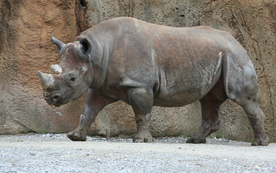
\includegraphics{rhino.jpg}
\end{frame}

\subsubsection{References}
\begin{frame}{References}
\begin{itemize}
\item Backcountry \url{http://www.backcountry.com/}
\item FragnanceNet \url{http://www.fragrancenet.com/}
\end{itemize}
\end{frame}

While there are still a lot of sites with Interchange around,
there are basically no new projects done with Interchange.

\subsection{Future}
\begin{frame}{Future}
  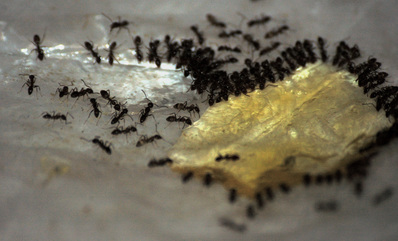
\includegraphics{ants.jpg}
\end{frame}

\subsubsection{Principles}
Examples for being agnostic:

The Cart class doesn't make assumptions where the items are
stored, they could be in the session or in the database.

The Account Manager class allows multiple authentication
methods through account providers.

We don't have a fixed templating system like in Interchange.

We are not tied to a certain framework.

\begin{frame}{Principles}
\begin{itemize}
\item KISS
\item Components
\item Agnostic
\item Expressive
\end{itemize}
\end{frame}

\begin{frame}{Agnostic}
Cart
\begin{itemize}
\item Session
\item DBI
\item Webservice *
\end{itemize}
\end{frame}

\begin{frame}{Agnostic}
Account Manager
\begin{itemize}
\item DBI
\item LDAP *
\item OpenID *
\end{itemize}
\end{frame}

\begin{frame}{Agnostic}
Templating Engine
\begin{itemize}
\item Template::Toolkit
\item Template::Flute
\end{itemize}
\end{frame}

\begin{frame}{Agnostic}
Web framework
\begin{itemize}
\item Catalyst
\item Mojo
\item Dancer
\end{itemize}
\end{frame}

To have these choices is good for developers and experienced users, 
but many users want to exactly know what they are getting.

Dancer fits our preferences the best.

Template::Flute allows us to use pure HTML templates.

DBI is the common storage method for Ecommerce products.

\begin{frame}{Preferences}
\begin{itemize}
\item Dancer
\item Template::Flute
\item DBI
\end{itemize}
\end{frame}

\subsubsection{Framework}
By using an existing web framework which is Plack/PSGI compatible
we get relieved of the following
tasks and gain more flexibility in
addition.
 
\begin{frame}{Framework}
\begin{itemize}
\item Dispatching requests
\item Parameter parsing
\item Session handling
\item Template engine
\item I18N
\end{itemize}
\end{frame}

\subsubsection{Extensions}
\begin{frame}{Extensions}
\begin{itemize}
\item Bundles
\item Plugins
\item Hooks
\end{itemize}
\end{frame}

\subsubsection{Features}
\begin{frame}{Features}
\begin{itemize}
\item Navigation
\item Cart
\item Checkout
\item Accounts
\end{itemize}
\end{frame}

% \subsection{How easy can it be?}
% \begin{frame}[fragile]{How easy can it be?}
% \begin{lstlisting}
% #!/usr/bin/env perl

% use Dancer;
% use Dancer::Plugin::Interchange;

% sell;
% \end{lstlisting}
% \end{frame}

% \subsection{Real World}
% Running and maintaining an online shop is a challenging business
% and requires constant change to stay on top of your competitors.

% \begin{frame}{Real World}
% \begin{itemize}
% \item Marketing, SEO
% \item Legal stuff
% \item Interfaces
% \item Design
% \end{itemize}
% \end{frame}

\section{API}
\subsection{Cart}
\begin{frame}{Cart}
\begin{itemize}
\item SKU, Name, Quantity, Price
\item Price > 0
\item Combines automatically
\item Multiple carts
\item Storage everywhere
\item Price caching
\end{itemize}
\end{frame}

\begin{frame}[fragile]{Nitesi::Cart Methods}
\begin{lstlisting}
use Dancer::Plugin::Nitesi;

cart->add(sku => 'POM253', name => 'Pomelo',
    price => 3.00, quantity => 10);

cart->remove(sku => 'POM253');

cart->count();

cart->clear();

cart->total();

cart->subtotal();
\end{lstlisting}
\end{frame}

\subsubsection{Everything is a Cart}
\begin{frame}{Everything is a Cart}
\begin{itemize}
\item Saved Carts
\item Wishlists
\item Collections
\end{itemize}
\end{frame}

\begin{frame}[fragile]{Multiple Carts}
\begin{lstlisting}
cart('wishlist')->add(sku => 'ORA322', name => 'Orange',
     price => 2.00, quantity => 5);

\end{lstlisting}
\end{frame}

\subsubsection{Cart Backends}
\begin{frame}{Cart Backends}
\begin{itemize}
\item Session
\item DBI
\end{itemize}
\end{frame}

\subsubsection{Inventory Checks}
Inventory checks are pretty much limited in Interchange right now.
They are controlled by the configuration directives MinQuantityField
and MaxQuantityField:
\begin{frame}[fragile]{Inventory Check}
\begin{lstlisting}
MinQuantityField min_quantity
MaxQuantityField inventory:quantity 
\end{lstlisting}
\end{frame}
Also they are part of the standard code instead of loaded through
hooks.

\begin{frame}[fragile]{Inventory Check Hook}
\begin{lstlisting}
hook 'before_cart_add' => sub {
    my ($cart, $item) = @_;
    my ($inventory);

    $inventory = query->select_field(table => 'products',
                                     field => 'inventory',
                                     where => {sku => $item->{sku}});
				     
    if ($item->{quantity} > $inventory) {
        $item->{error} = 'Out of stock';
    }
};
\end{lstlisting}
\end{frame}

\subsubsection{Cart Hooks}
We just seen an example for before_cart_add hook.

The most common usage for after_cart_add is to update the cart
in the backend storage, for example storing the new item in the tables 
used by the DBI backend and update the modification date of the cart.

\begin{frame}{Cart Hooks}
\begin{itemize}
\item before\_cart\_add
\item after\_cart\_add
\end{itemize}
\end{frame}

after_cart_remove is used in a similar way as after_cart_add 
for removing the item in the tables used by the DBI backend
and update the modification date of the cart.

\begin{frame}{Cart Hooks}
\begin{itemize}
\item before\_cart\_remove
\item after\_cart\_remove
\end{itemize}
\end{frame}

\subsection{Checkout}

\begin{frame}{Checkout}
\begin{itemize}
\item Taxes
\item Shipping
\item Payment
\item Invoice
\end{itemize}
\end{frame}

\subsubsection{Payment}
\begin{frame}{Payment}
\begin{itemize}
\item Business::CreditCard
\item Business::OnlinePayment
\end{itemize}
\end{frame}

\subsubsection{Taxes}
Tax on top of the product cost can be applied in different varieties.

Germany has 19\% salestax, 7.5\% reduced salestax for books and some
items are tax free. You have to show the breakdown of different taxes
on the receipt.

Orders for businesses between different countries of the EU are exempt
of salestax if the buying party has a salestaxid.

Business::Tax::VAT doesn't account for reduced rates.

\begin{frame}{Tax Modules on CPAN}
\begin{itemize}
\item Business::Tax::Canada
\item Business::CA::GST
\item Business::Tax::VAT
\item Business::Tax::VAT::Validation
\end{itemize}
\end{frame}

\subsubsection{Shipping}
\begin{frame}{Shipping}
\begin{itemize}
\item Simple Shipping
\item Crazy Shipping
\item Shipping API
\end{itemize}
\end{frame}

\subsubsection{Costs}
\begin{frame}[fragile]{Costs}
\begin{lstlisting}
$cart->apply_cost(amount => 5);

$cart->apply_cost(amount => 0.19, relative => 1);
\end{lstlisting}
\end{frame}

\subsubsection{PDF Invoices}
\begin{frame}{PDF Invoices}
\begin{itemize}
\item HTML template
\item Template::Flute::PDF
\end{itemize}
\end{frame}

\subsection{Accounts and Access Control}

\begin{frame}[fragile]{Accounts}
\begin{lstlisting}
post '/login' => sub {
    if (account->login(username => params('body')->{username},
                       password => params('body')->{password})) {
        redirect '/customerservice';
    }
    else {
        redirect '/login';
    }
};
\end{lstlisting}
\end{frame}

\begin{frame}[fragile]{Accounts}
\begin{lstlisting}
get '/checkout' => sub {
    if (account->acl(check => 'submit_orders')) {
        return template 'checkout';
    }
    
    redirect '/access_denied';
};
\end{lstlisting}
\end{frame}

\subsubsection{Account Manager}
\begin{frame}{Account manager}
\begin{itemize}
\item Account Providers
\item Login/Logout
\item Account Information
\item Login status
\item Forgot password
\item Registration
\end{itemize}
\end{frame}

\subsubsection{Account Provider}
\begin{frame}{Account Provider}
\begin{itemize}
\item DBI 
\item LDAP *
\item Htpasswd * 
\item OpenID *
\item OAuth *
\end{itemize}
\end{frame}

\subsubsection{Access Control}
\begin{frame}{Access Control}
\begin{itemize}
\item User
\item Roles
\item Permissions
\end{itemize}
\end{frame}

\subsection{Forms}
\begin{frame}{Forms}
\begin{itemize}
\item Display
\item Validation
\item Storage
\end{itemize}
\end{frame}

\subsection{Web Services}
\begin{frame}{Web Services}
\begin{itemize}
\item REST
\item XML-RPC
\item SOAP
\end{itemize}
\end{frame}

\section{Development \& Deployment}
\subsection{Dancer}
\subsubsection{Routes}
\begin{frame}{Routes}
\begin{itemize}
\item Categories
\item Products
\item Cart
\item Checkout
\item Login/Logout
\item Customer Service
\end{itemize}
\end{frame}

\subsubsection{Default Route}
Categories and products can be handled through the default route
(see
\url{http://search.cpan.org/~sukria/Dancer/lib/Dancer/Cookbook.pod#Default_route})
as alternative to defining explicit routes.

\begin{frame}[fragile]{Default Route}
\begin{lstlisting}
get qr{/(.*)} => sub {
    my ($sku) = splat;
    my $product;

    # check for existing product
    if ($product = database->quick_select('products', {sku => $sku})) {
        # display flypage
        template 'flypage', $product;
    }
    else {
        # display not found page
        status 'not_found';
        forward '404';
    }
};
\end{lstlisting}
\end{frame}

\subsection{Contribution}
\subsubsection{Nitesi @ CPAN/GitHub}
\begin{frame}{CPAN/GitHub}
\begin{itemize}
\item \url{http://search.cpan.org/dist/Nitesi/}
\item \url{http://search.cpan.org/dist/Nitesi-DBI/}
\item \url{http://search.cpan.org/dist/Dancer-Plugin-Nitesi/}
\end{itemize}
\begin{itemize}
\item \url{https://github.com/racke/Nitesi}
\item \url{https://github.com/racke/Nitesi-DBI}
\item \url{https://github.com/racke/Dancer-Plugin-Nitesi}
\end{itemize}
\end{frame}

\subsection{The End}
\begin{frame}{The End}
Slides:
\url{http://www.linuxia.de/talks/perlcommerce/perlcommerce-beamer.pdf}

Project:
\url{https://vsc.state.gov/}
\end{frame}
\end{document}

%%% Local Variables: 
%%% mode: latex
%%% TeX-master: t
%%% End: 
